

\section{Additional Results}
\label{sec:extra_results}

\subsection{Ablation: Using Prediction Market Binary Data}
\label{sec:binary_ablations}



\begin{figure}[h]
  \centering
  \begin{subfigure}[t]{0.98\textwidth}
    \centering
    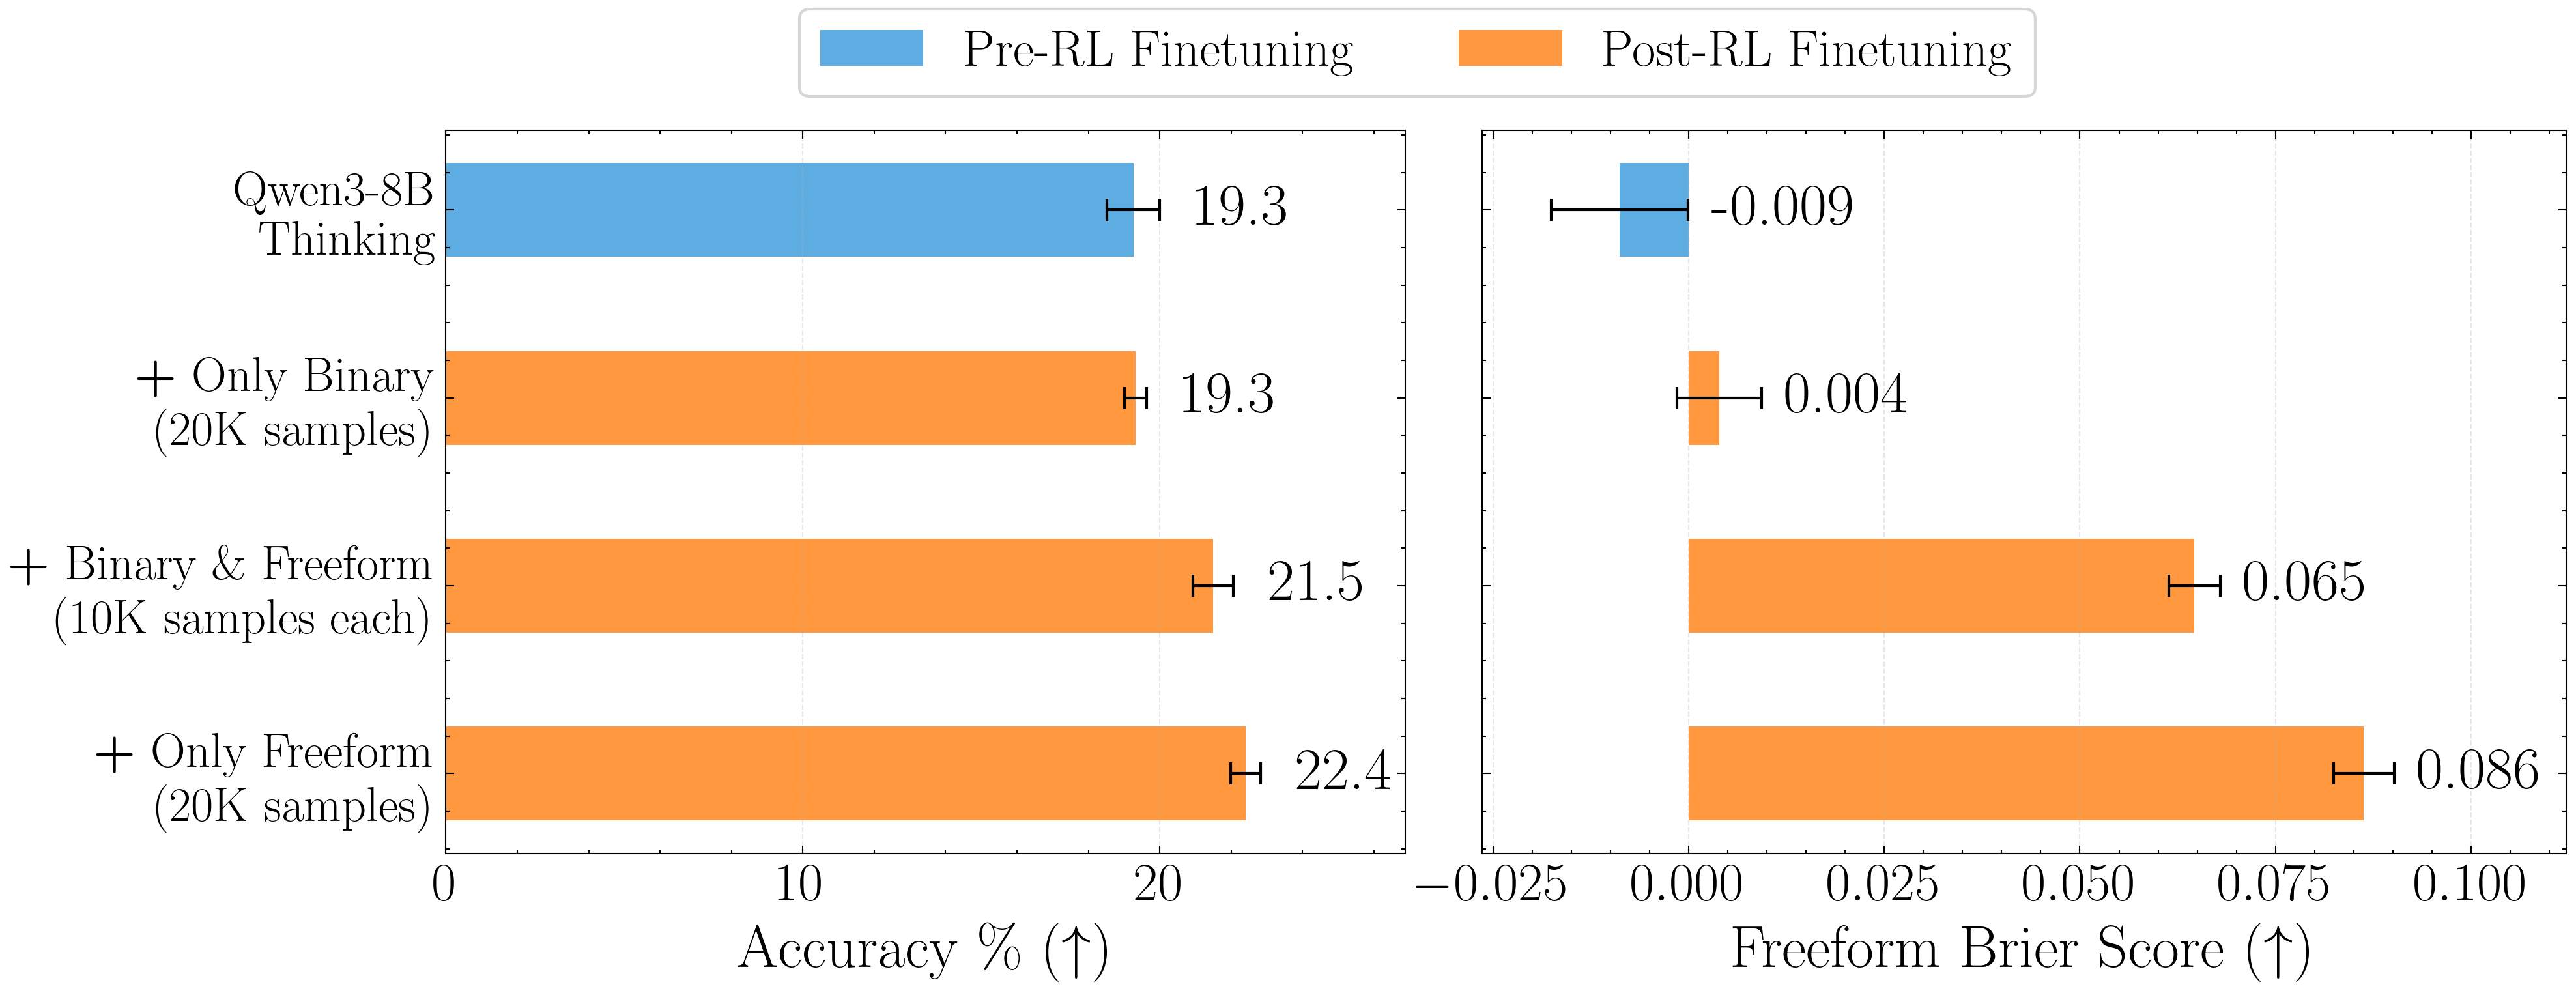
\includegraphics[width=\linewidth,keepaspectratio]{figures/binary_ablations/theguardian-july-ablations.png}
    \caption{Performance on our \textbf{Validation Set} composed of question from TheGuardian news source from July 2025.}
    \vspace{0.3cm}
    \label{fig:binary_ablations_guardian}
  \end{subfigure}
  \hfill
  \begin{subfigure}[t]{0.98\textwidth}
    \centering
    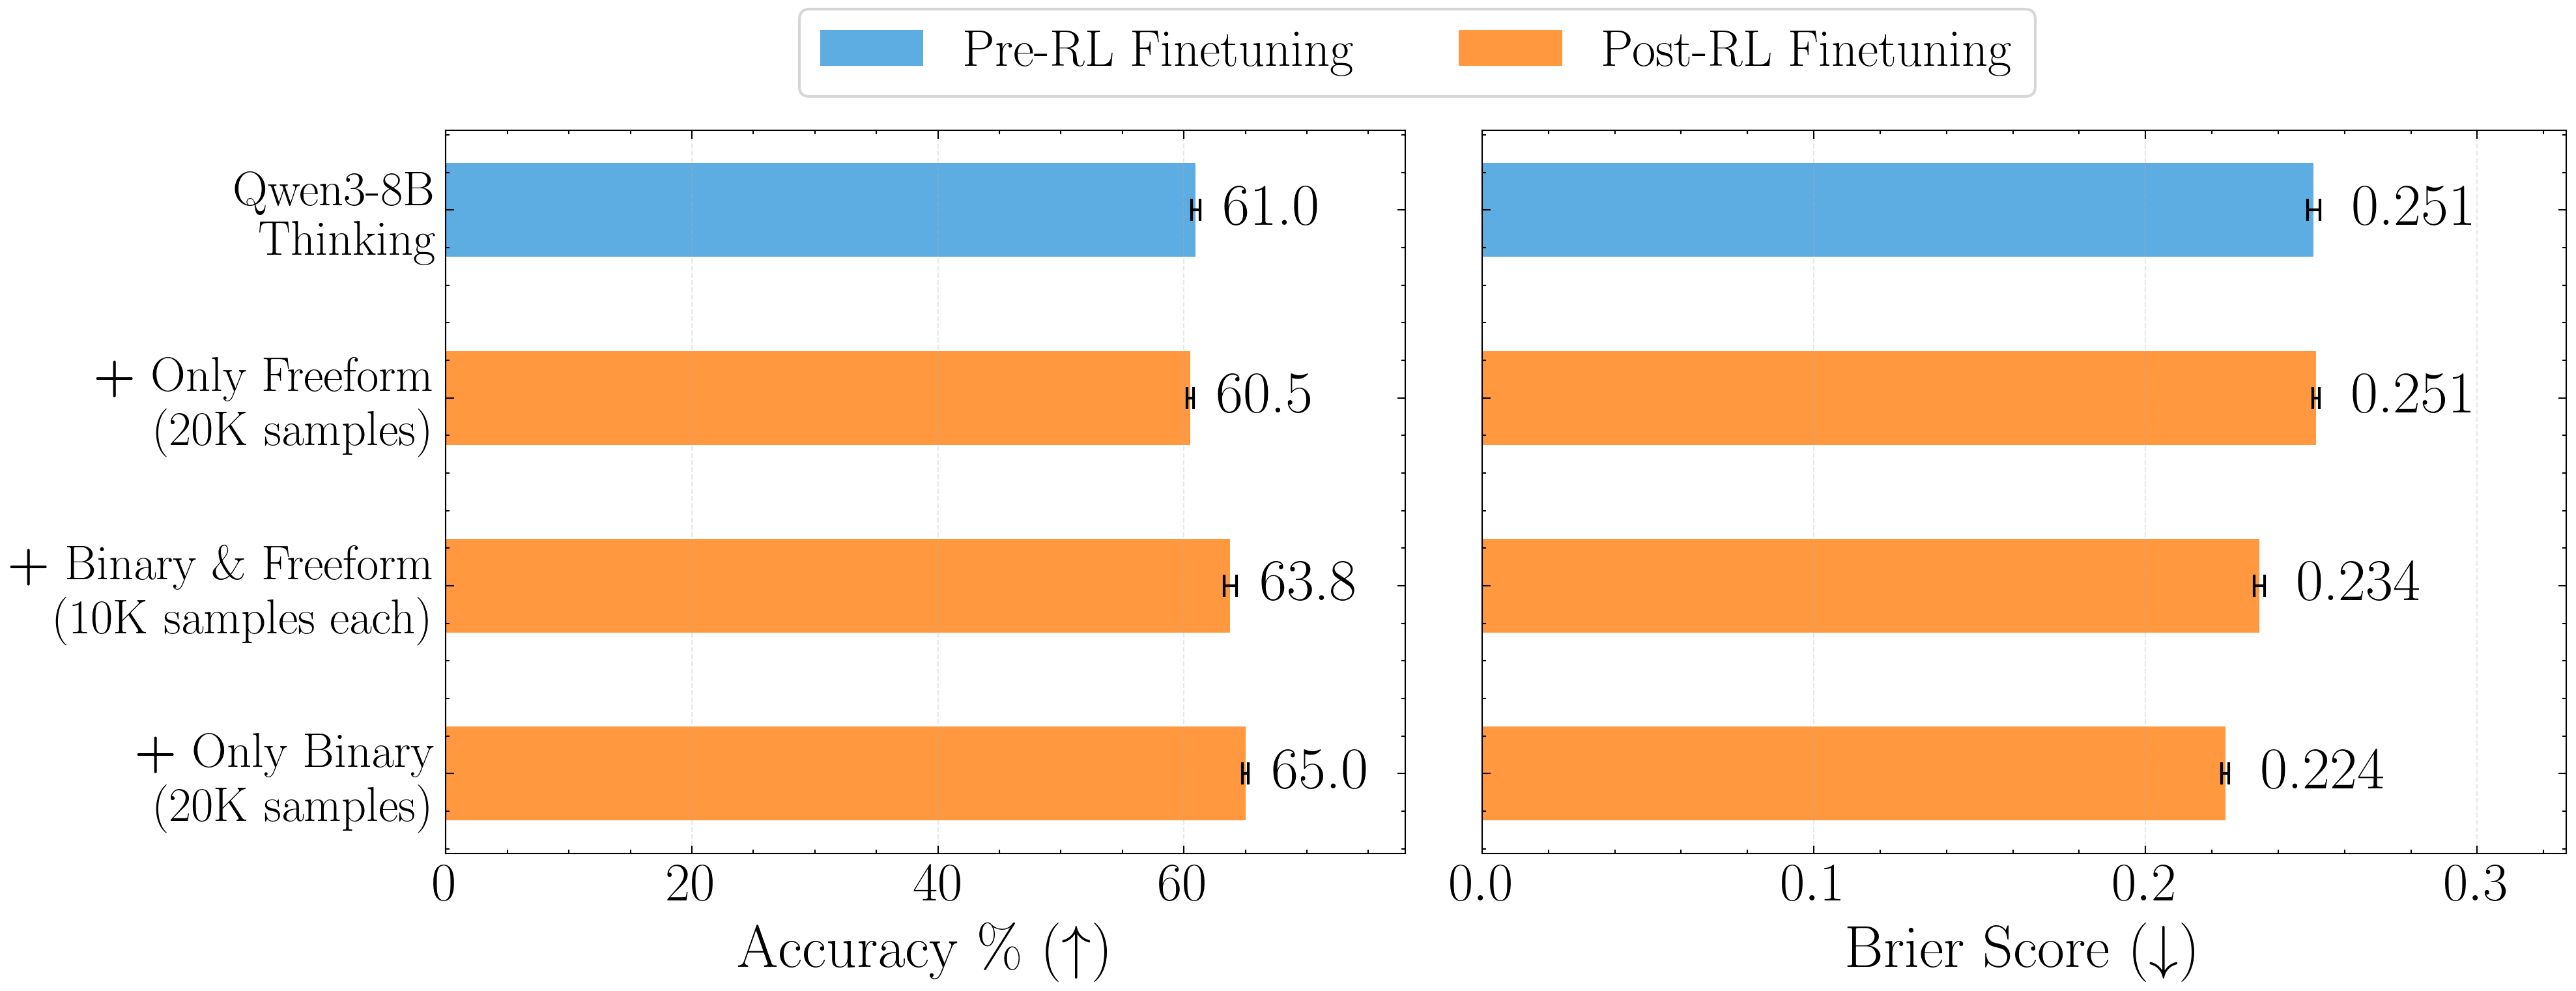
\includegraphics[width=\linewidth,keepaspectratio]{figures/binary_ablations/metaculus-ablations.png}
    \caption{ Performance on \textbf{Metaculus binary} questions resolved in May–July 2025.}
    \label{fig:binary_ablations_metaculus}
  \end{subfigure}

  \caption{\looseness -1 \textbf{Performance of different data ablations.} 
  We evaluate performance after training on 3 different supervision signals: 
  (i) only binary data (20K samples), 
  (ii) only freeform data (20K samples), and 
  (iii) both binary and freeform data (10K samples each) for data-matched comparison. 
  (a) Accuracy and freeform Brier score of the initial and post-RL model on our Validation Set from July 2025. 
  (b) Accuracy and binary Brier score of initial and post-RL model on volume-filtered binary questions resolved between May and July 2025 on Metaculus. 
  \textit{We find training on binary questions hurts performance on open-ended forecasting, but is necessary to retain performance on binary prediction market questions.}}
  \label{fig:binary_ablations}
\end{figure}


We ablate supervision type with \texttt{Qwen3-8B} using three size-matched settings (Figure~\ref{fig:binary_ablations}). For \emph{binary-only}, we curate \textbf{20K} resolved markets from Manifold, volume-filtered to ensure engagement; because many markets resolve slowly, this set spans the past five years. For \emph{free-form only}, we use \textbf{20K} pipeline-generated, usable questions from Forbes articles. For the \emph{binary+free-form mix}, we take \textbf{10K} Manifold + \textbf{10K} Forbes questions to keep total examples constant. The goal is to isolate which \emph{learning signal}---binary resolution vs.\ open-ended outcome specification---most effectively trains calibrated forecasters under identical compute and token budgets.

On the free-form test set (Fig.~\ref{fig:binary_ablations} Left), post-RL performance improves most with \emph{free-form only} supervision (Accuracy \(19.3\%\!\rightarrow\!22.4\%\); Free-form Brier \(-0.009\!\rightarrow\!0.086\)). Mixing binary and free-form also helps (Brier \(0.065\)), whereas \emph{binary-only} yields minimal gains on free-form evaluation (Brier \(0.004\)). On Metaculus (binary) (Fig.~\ref{fig:binary_ablations} Right), both \emph{binary-only} and the \emph{mixed} setting improve accuracy and Brier, with the \emph{binary+free-form} mix offering the best overall trade-off across testing formats. Our gains by training on binary-only format are consistent with prior work by \citet{turtel2025outcome, turtel2025llms}. However, we do not arrive at a single unanimous recipe: free-form data is essential for open-ended forecasting, while combining formats appears Pareto-optimal across binary and free-form evaluations. Practically, it seems training on a \emph{mixture} of question styles provides the most robust gains across tasks.


% \subsection{Ablation: Effects of Supervised Finetuning}


\subsection{Varying models and evaluation months}
\label{sec:extra_forecasting_results}

\begin{wrapfigure}[18]{r}{0.5\textwidth} % 'r' for right, 0.4\textwidth for width of figure area
    % \vspace{-0.4cm}
    \centering
    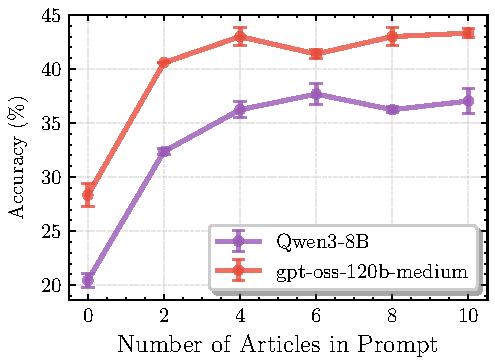
\includegraphics[width=0.95\linewidth]{figures/retrieval/varying_articles_accuracy_Llama_4_Scout.pdf}
    \caption{\textbf{Improvements from retrieval plateau at $\sim 5$ chunks.} We show the accuracy of both a large GPT-OSS-120B model and a small Qwen3-8B model which we finetune.}
    \label{fig:articles_retrived}
    % \vspace{-.2cm} % latex is overrating the gap
\end{wrapfigure}


In ~\Cref{fig:articles_retrived} we observe that while the first few article chunks that are retrieved lead to large improvements, at around five articles, improvements plateau, both on our Qwen3-8B and also other large models like GPT-OSS-120B. Thus, unless otherwise specified, we use 5 articles for all evaluations and training in this work. 


\paragraph{Improvement on non-Qwen models.} 
Our training data \ourdataset \ can be used to improve models across different families. In Figure~\ref{fig:extramodels_performance} we show improvements for Llama-3.1-8B-Instruct, Llama-3.2-3B-Instruct and Gemma-3-4B-Instruct. We see particularly large improvements in both accuracy and Brier score for Llama due to both: poor initial performance, but also surprising amenability to RL training with our data as the final performance exceeds much larger models like Qwen3-235B-A22B and DeepSeek-v3. %We also provide a qualitative analysis of the change in performance of Llama-3.1-8B in \Cref{sec:qualitative_analysis}.

% 

\begin{figure}[h]
    \centering
    
    \begin{minipage}[t]{0.48\textwidth}
        \centering
        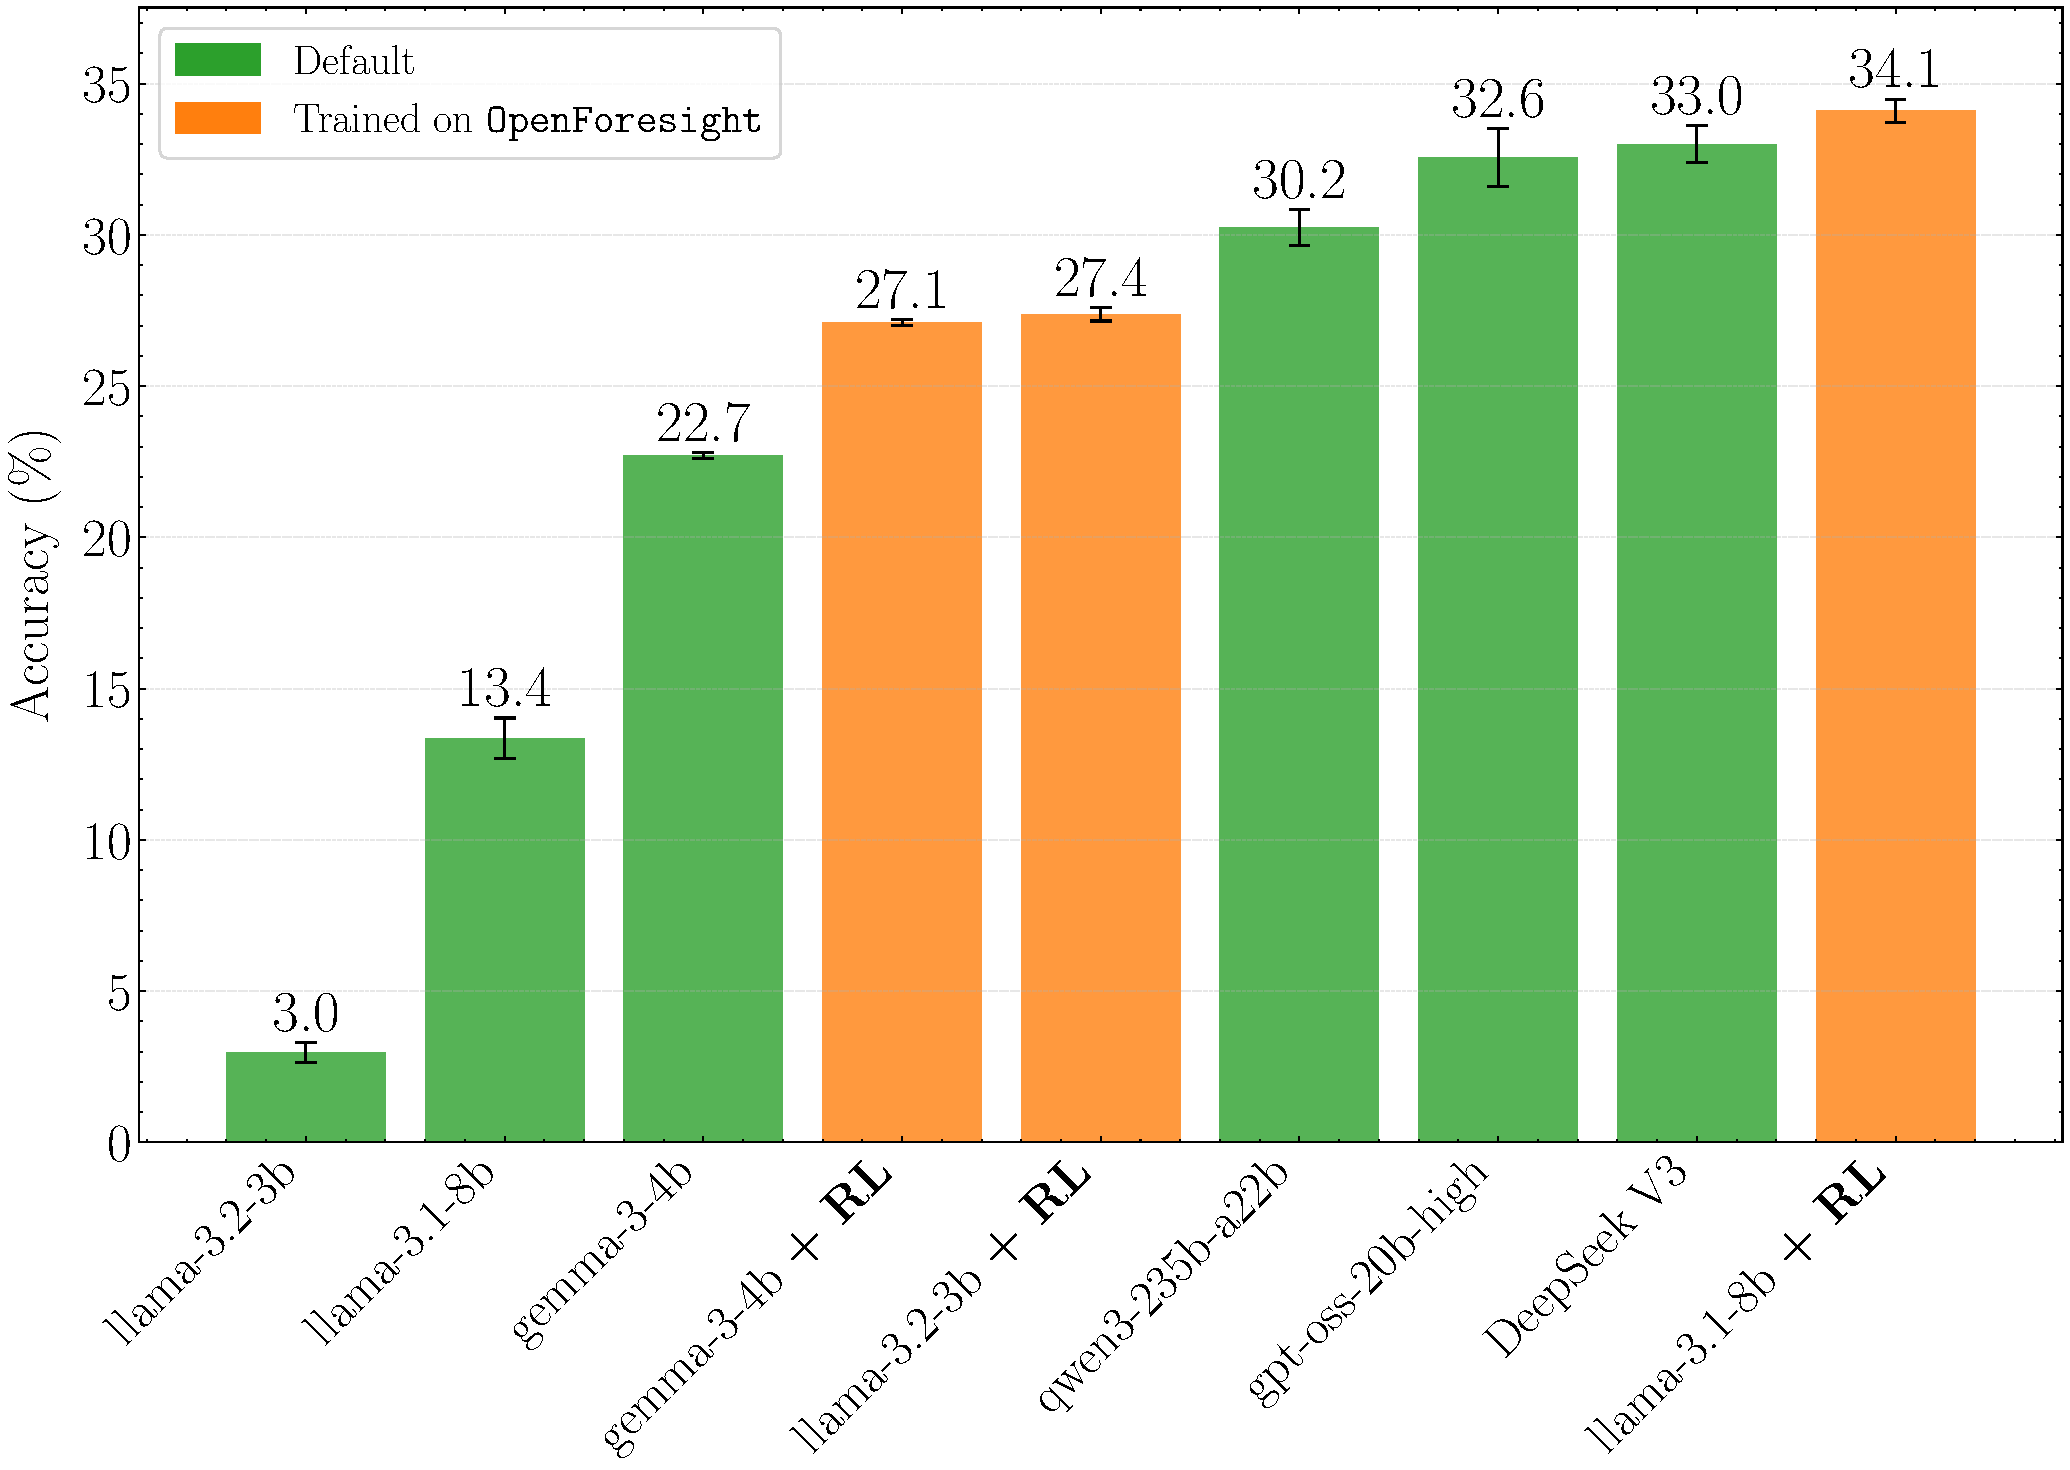
\includegraphics[width=\linewidth]{figures/testset-final/others/accuracy_others_Llama_4_Scout.pdf}
        % \caption{{Accuracy of the models on FutureX Past.} }
        % \label{fig:futurex_acc}
         % latex is overrating the gap
    \end{minipage}
    \begin{minipage}[t]{0.48\textwidth}
        \centering
        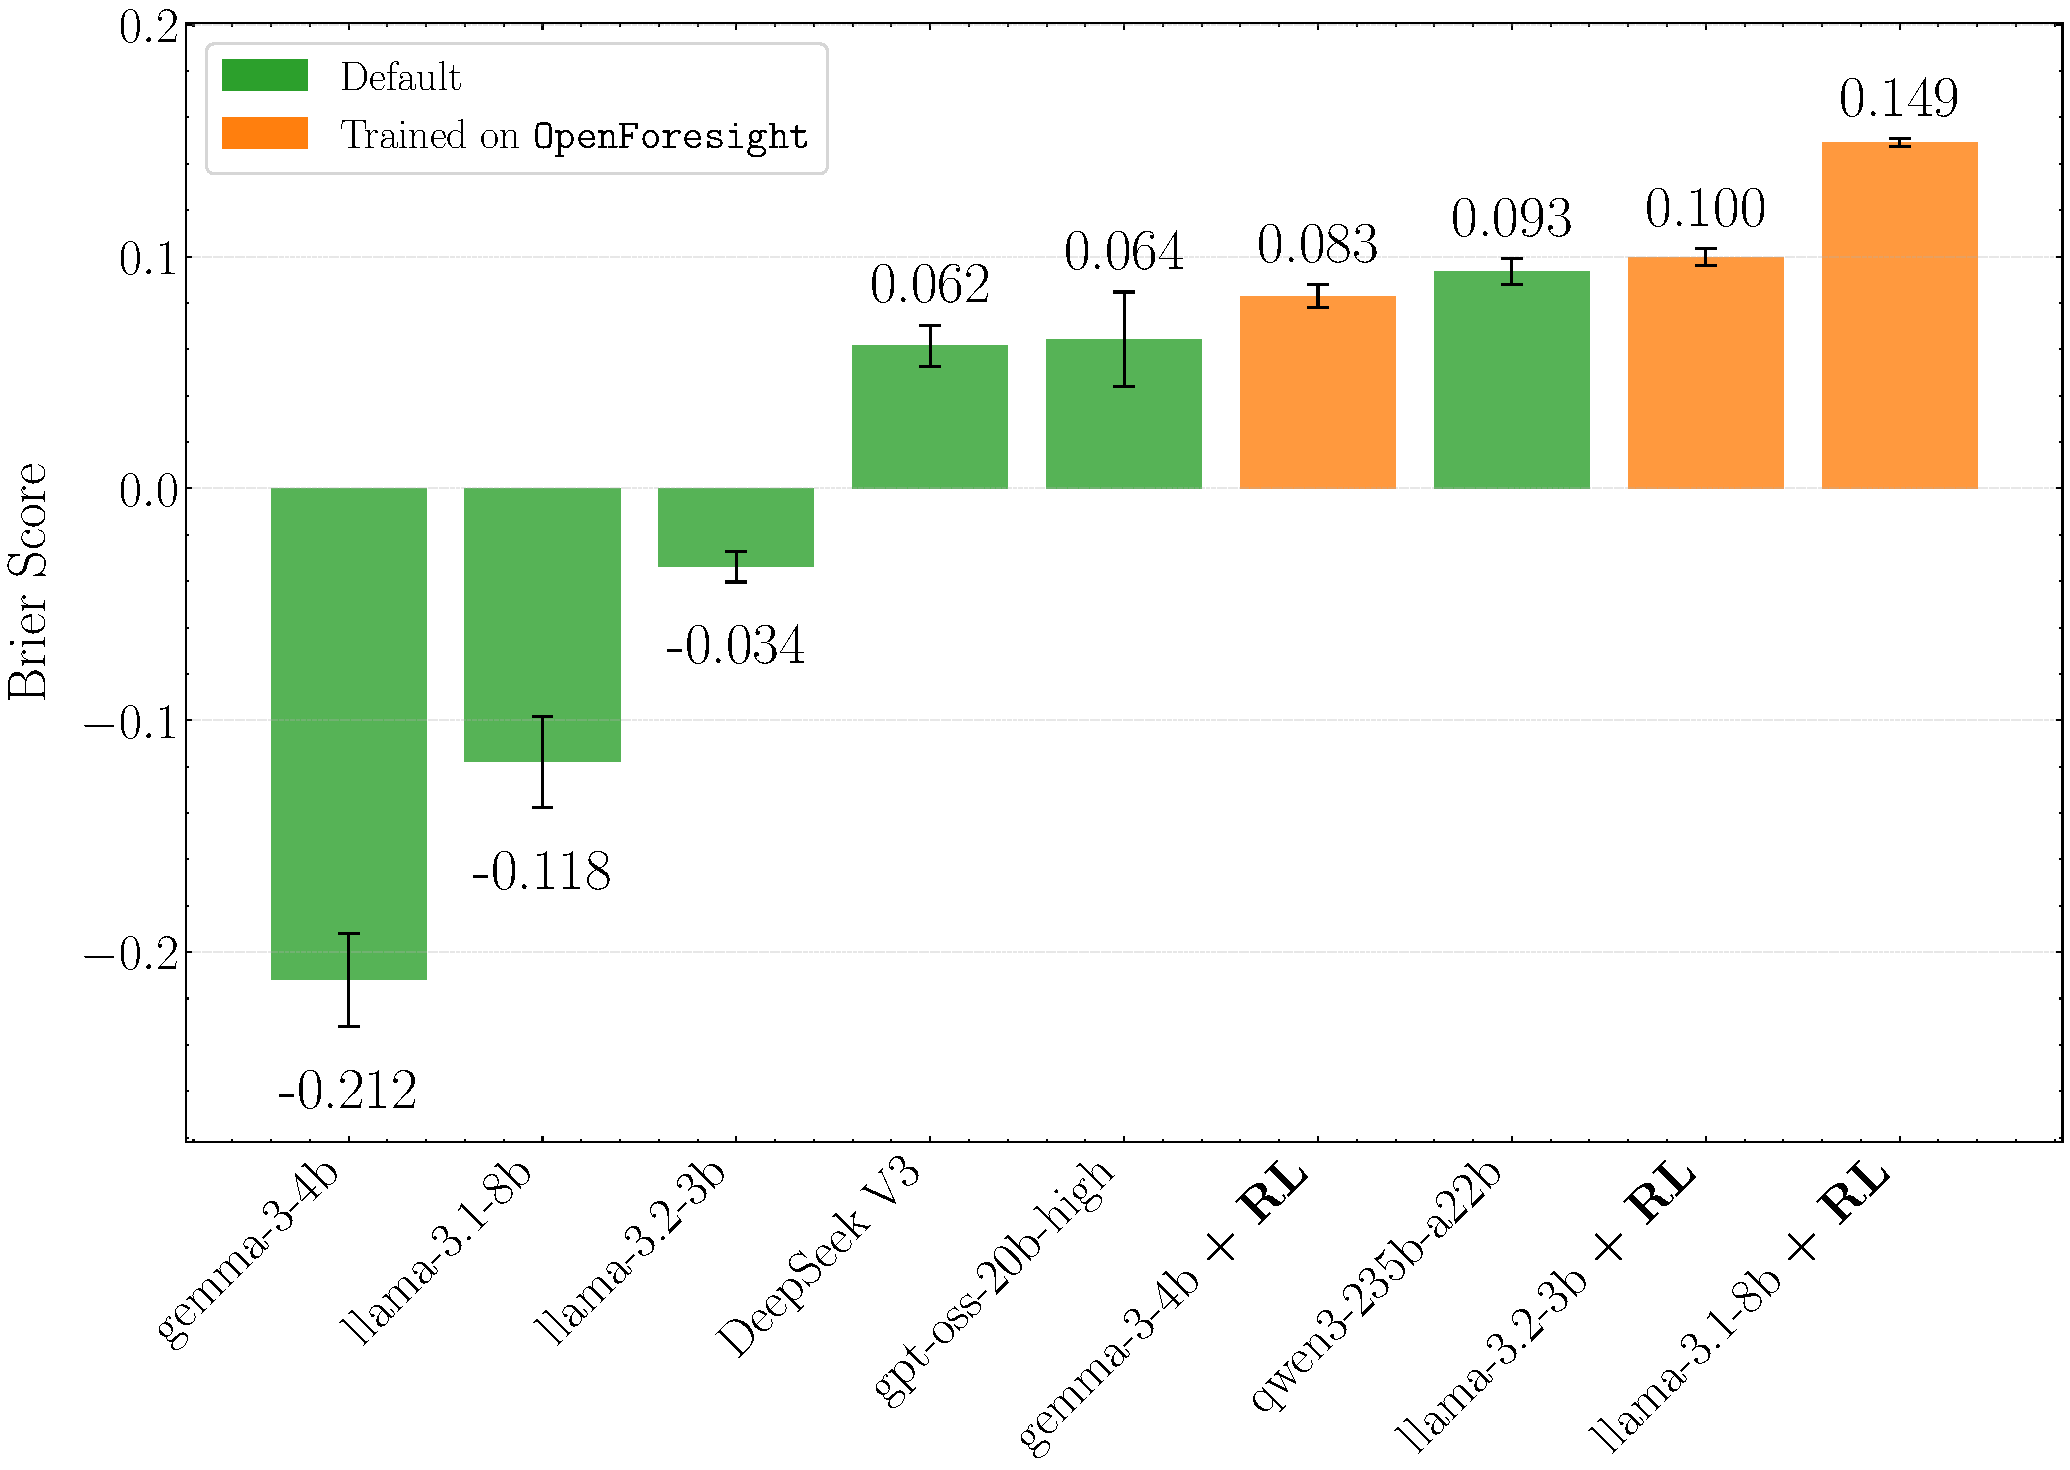
\includegraphics[width=\linewidth]{figures/testset-final/others/brier_scores_others_Llama_4_Scout.pdf}
        % \caption{{Brier Score of the models on FutureX Past benchmark.} }
        % \label{fig:futurex_brier}
        \vspace{-.2cm} % latex is overrating the gap
    \end{minipage}
    
    \caption{Performance of models from Llama and Gemma family on our test set.} 
    \label{fig:extramodels_performance}
\end{figure}



\begin{figure}[h]
    \centering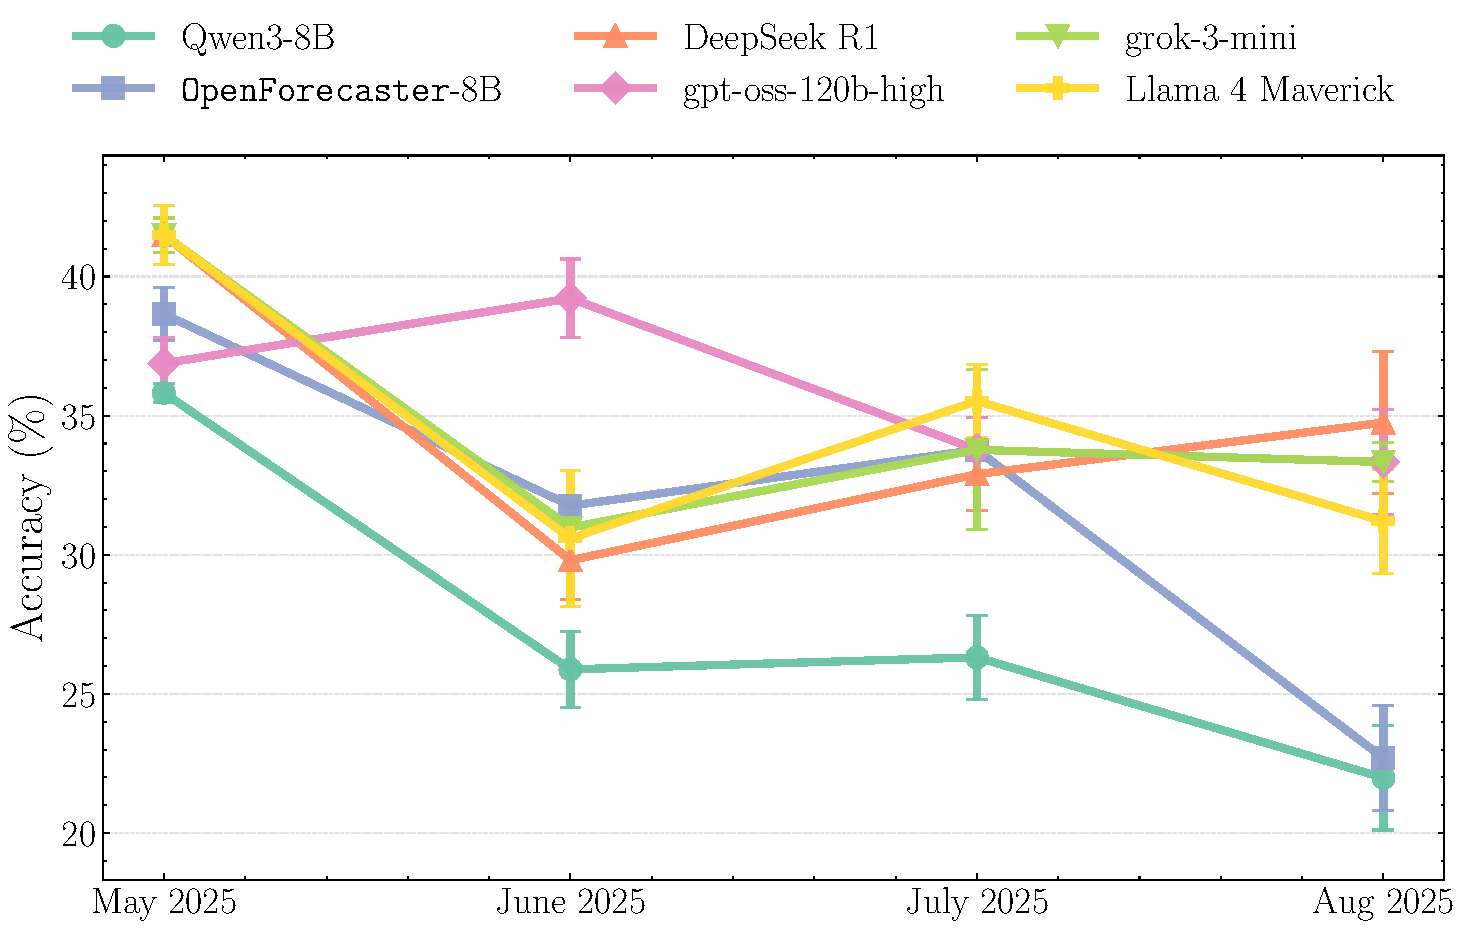
\includegraphics[width=0.75\linewidth]{figures/testset-final/monthly/accuracy_by_month_testset-monthly_Llama_4_Scout.pdf}
        \caption{{Monthly accuracy of the models on our test set.} }
        \label{fig:monthly_accuracy}
        \vspace{0.2cm}
    
  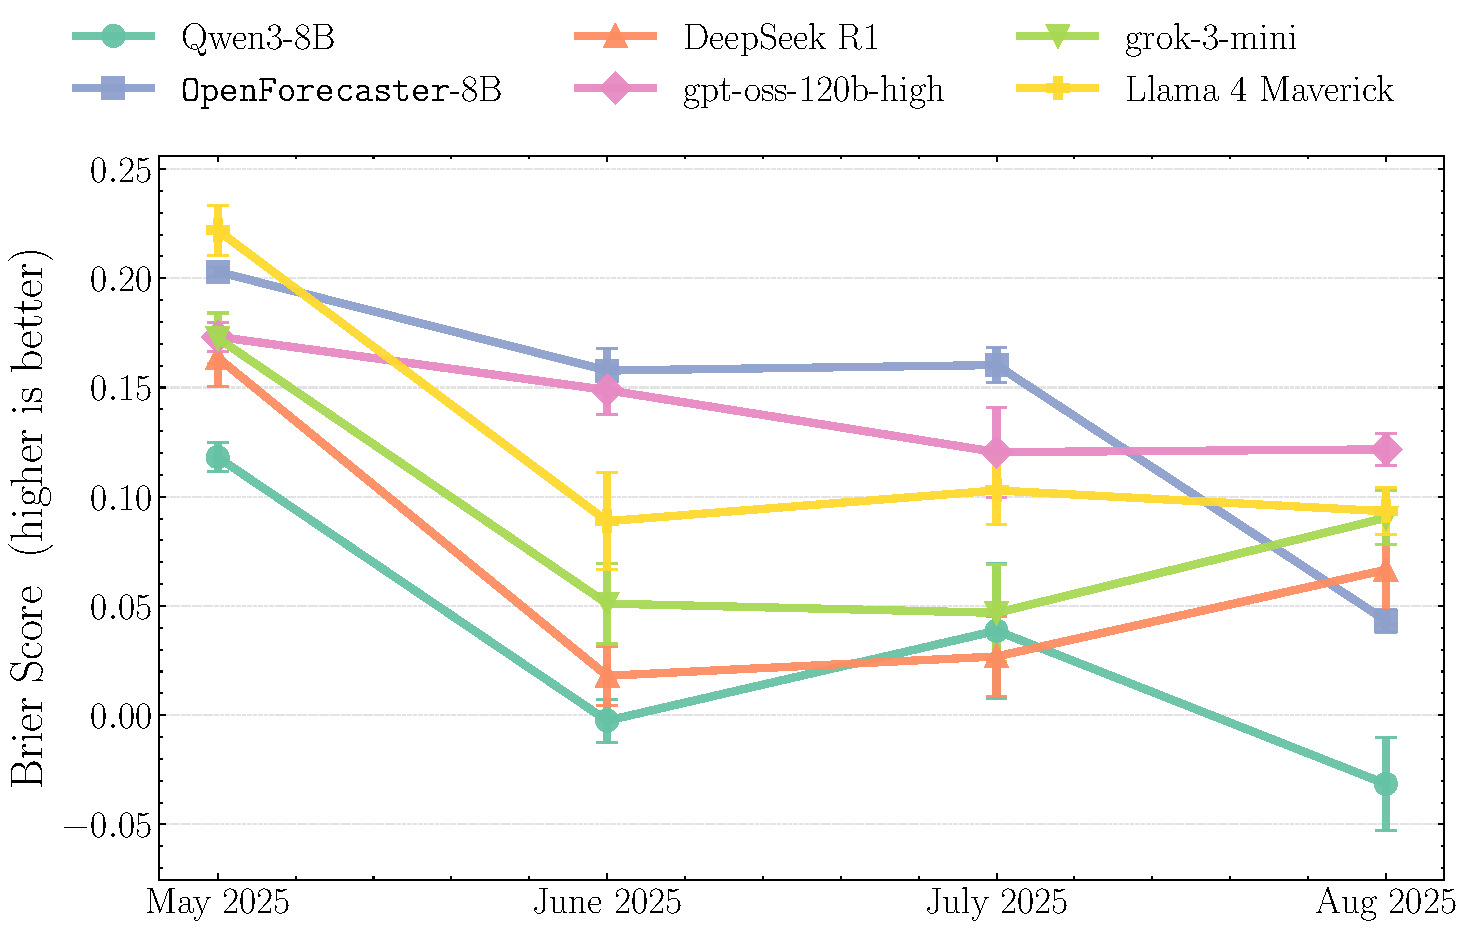
\includegraphics[width=0.75\linewidth]{figures/testset-final/monthly/brier_by_month_testset-monthly_Llama_4_Scout.pdf}
    \caption{{Monthly Brier score of the models} }
    \label{fig:monthly_brier}
    \vspace{-.2cm} % latex is overrating the gap
\end{figure}



\paragraph{Results over time.} As our test set is derived from articles from May to August 2025, so we split the questions by resolution date to get monthly performance of the models. Breaking down by month, our test has 94 questions resolving in May, 85 in June, 76 resolving in July and 47 resolving in August. We have lower number of questions in later months due to our filtering strategy for addressing late reporting in news. We first generated roughly equal number of questions per month and post-hoc filtered the ones whose true resolution date (found using grok-4.1-fast with search) was before May'25. 

For monthly performance, our hypothesis is that as we go further into the future, forecasting should become more difficult leading to lower performance. In \Cref{fig:monthly_accuracy} and \Cref{fig:monthly_brier}, we find that the accuracy and brier score of the models indeed drops gradually month-by-month consistent with our hypothesis. We also find that our trained models are consistently better than the original versions and also better than all other models in Brier score.




\subsection{Ablation with Supervised Finetuning}
\label{sec:sft_ablation}



\vspace{-.2cm}
% \paragraph{Supervised Finetuning (SFT).} 
Here we study what would be the benefit if we add a supervised finetuning (SFT) stage in our training process? While we start from the RL trained Qwen3 thinking models, they are far behind proprietary models as shown in~\Cref{fig:theguardian_retrieval_acc}. Several frontier model training reports~\citep{guo2025deepseek} mention using an SFT stage as a warm start before RL. We choose Grok-3-Mini to generate forecasting reasoning traces for SFT, as it has high performance, low cost, and provides the full reasoning trace through the API. 
% has low cost and high performance on our validation set and on external forecasting benchmarks like ProphetArena \citep{li2025we}. %like FutureX \citep{zeng2025futurex}.
Specifically, we construct a dataset of 10,000 questions from \textit{The Guardian} dated January–March 2025, beyond Grok-3-mini's reported knowledge cutoff of June 2024. Obtaining Grok-3-Mini's reasoning traces on this data costed $15$ USD. For distillation, we randomly choose the number of articles to put in its prompt (0 to 10) so that the student model can reason with any number of articles.  %To test the usefulness of SFT for eventual GRPO, we compute pass@k accuracy~\citep{wu2025invisibleleashrlvrescape}, which measures the fraction of samples where the model gets at least one attempt out of $k$ correct. 
% \citet{wu2025invisibleleashrlvrescape} show this is a useful indicator for amenability to improvements from GRPO.

Finally, we train this distilled checkpoint with GRPO using same data mixture, reward design and configurations as we used in training \ourmodel-8B. We report the results for both just distillation (Qwen3-8B-sft) and RL on the SFT checkpoint (as Qwen3-8B-sft-rl) in \Cref{fig:sft_test_set_performance} on our curated test set from May to August 2025. The final model achieves higher accuracy and much better calibration albeit with a slightly lower brier score. 

% Obtaining 10,000 reasoning traces from Grok-3-Mini for distillation costed $15$ dollars. 

% \footnote{These dates fall beyond Grok-3-Mini’s reported knowledge cutoff: although released in February 2025, the model reports a June 2024 cutoff when prompted.}.

% We apply supervised fine-tuning (SFT) for two reasons. First, SFT warm-starts reinforcement learning (RL), a practice several frontier model-training studies report as helpful \cite{}. Second, SFT lets us measure gains from training only on the forecasting task \cite{trainontesttask?}, isolating the effect of scaling the supervised signal. We use Grok-3-Mini for its performance, cheap cost, and open reasoning traces. We collect its reasoning traces for our questions and train with SFT. 



\begin{figure}[t]
\vspace{-0.25cm}
    \centering
    % Legend
    
\includegraphics[width=0.9\linewidth]{figures/sft/sft_scatter_brier_accuracy_test5news_302_Llama_4_Scout_legend.pdf}
    \hfill

    % (a) left plot
    \begin{subfigure}[t]{0.49\textwidth}
        \centering
        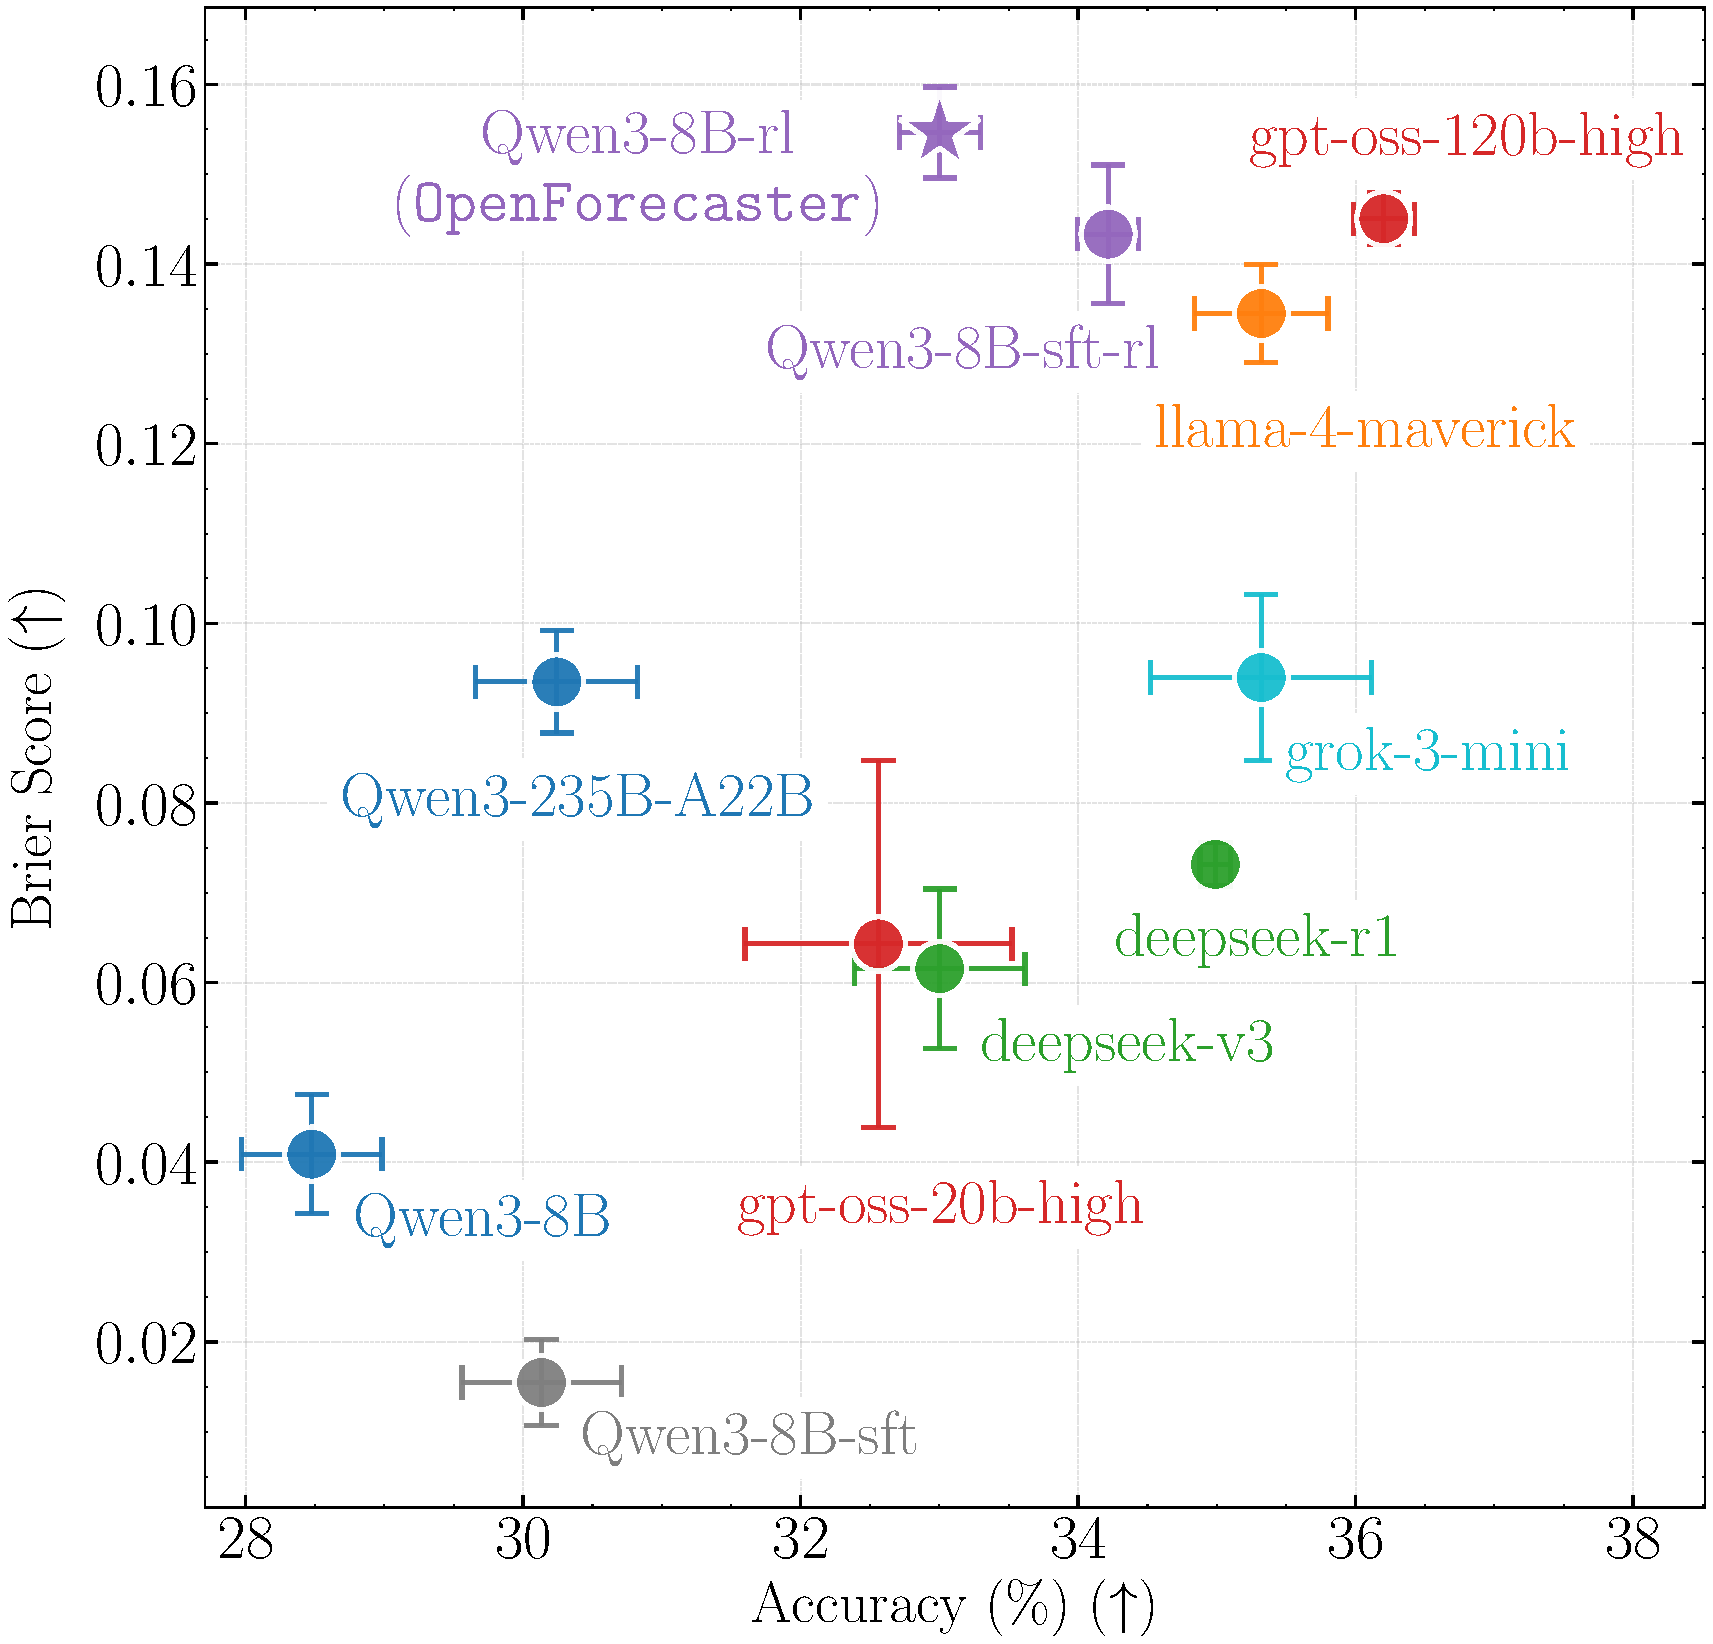
\includegraphics[width=0.9\linewidth]{figures/sft/sft_scatter_brier_accuracy_test5news_302_Llama_4_Scout.pdf}
        \caption{Results on our curated test set.}
        \label{fig:sft_test_set_performance}
    \end{subfigure}
    \hfill
    % (b) right plot
    \begin{subfigure}[t]{0.49\textwidth}
        \centering
        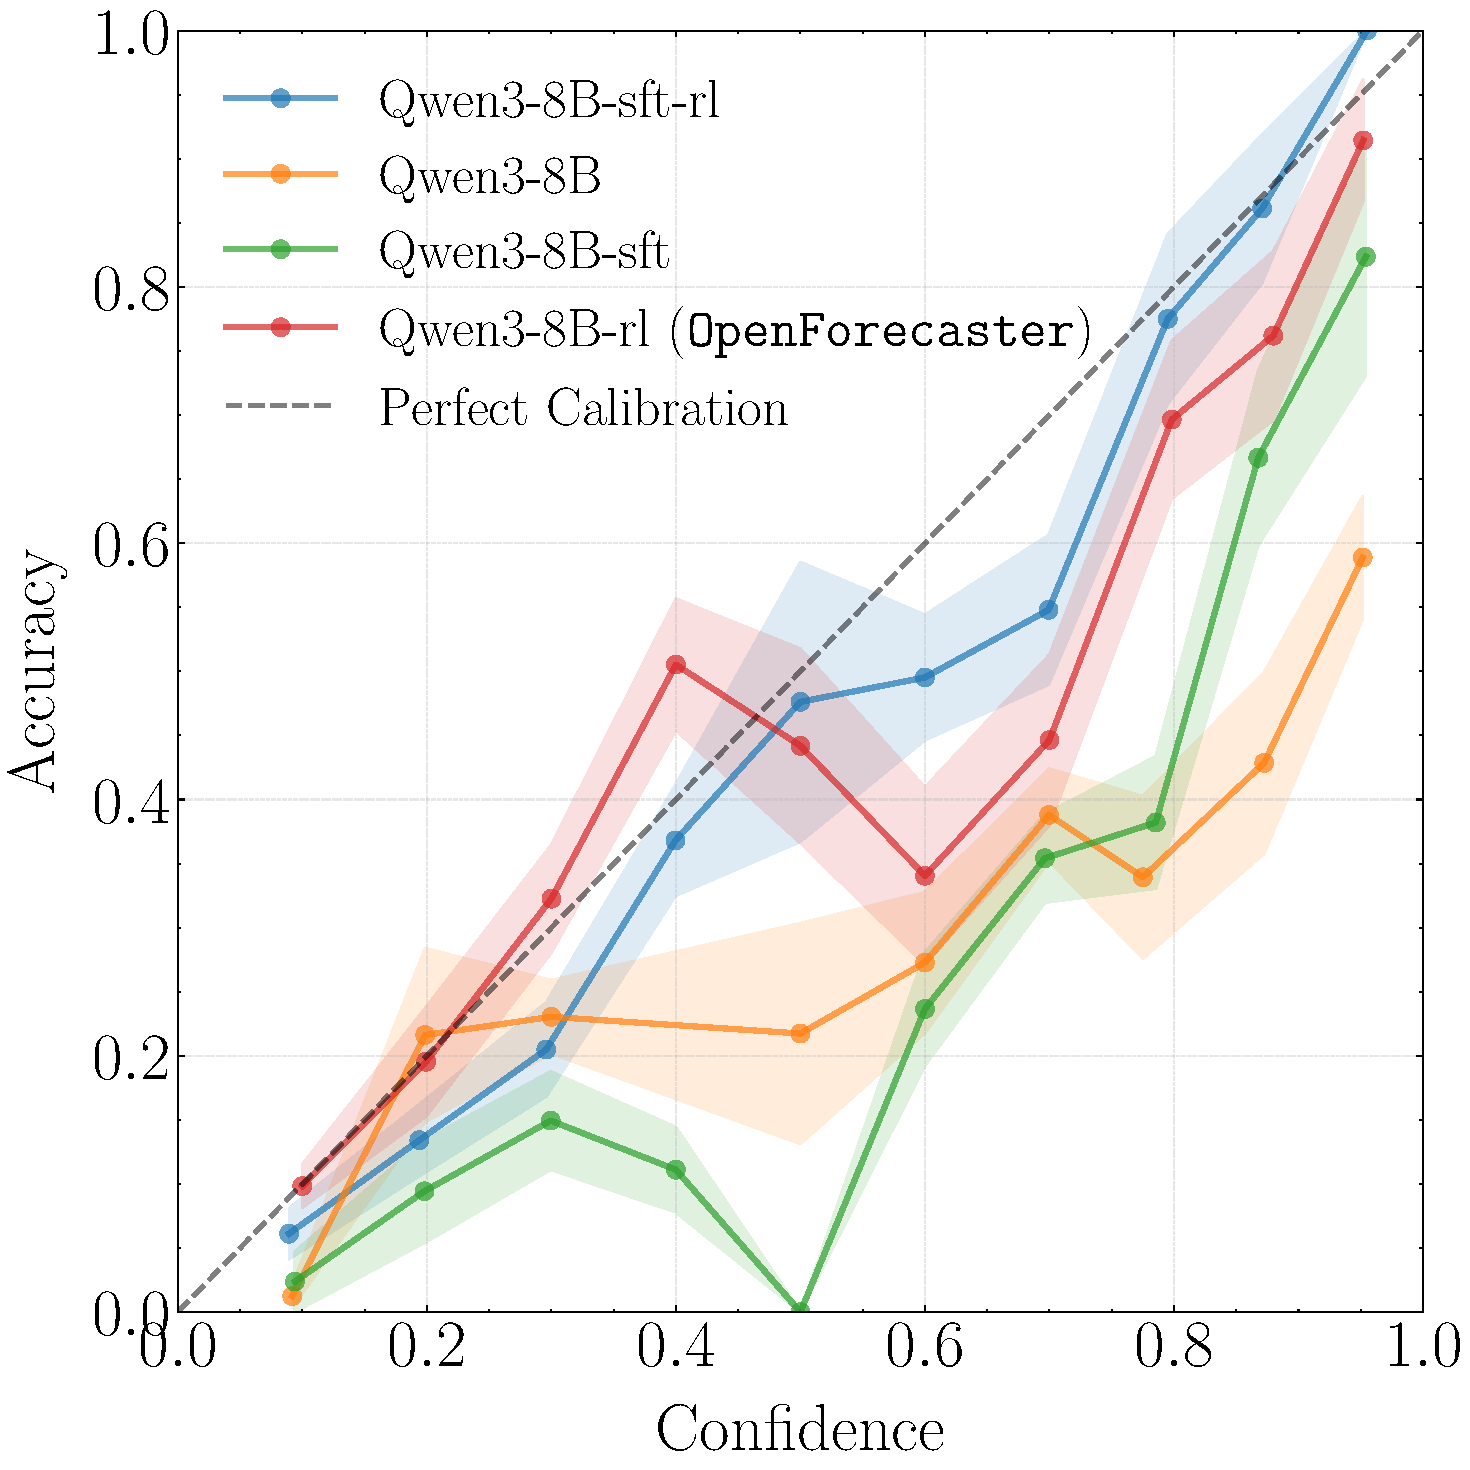
\includegraphics[width=0.9\linewidth]{figures/sft/calibration_all_qwen3_models_sft.pdf}
        \caption{ 
            Calibration curve of the models on our test set.
             }
        \label{fig:sft_calibration}
    \end{subfigure}

    \caption{
        RL training on \ourdataset \  improves the SFT models on accuracy. In particular, the calibration of Qwen-8B-sft-rl model (blue line) is near perfect. 
    }
    \vspace{-.2cm}
\end{figure}

% \subsection{Consistency Evaluation}
% \label{sec:consistency}
% \begin{table}[htbp]
% \centering
% \caption{\textbf{Improvement in consistency checks before and after RL training}. We report average violation scores and relative improvements (negative percentages indicate improvements). The RL-trained model shows substantial improvements in logical consistency across most reasoning tasks.}
% \label{tab:consistency_comparison}
% \resizebox{\textwidth}{!}{%
% \begin{tabular}{l|ccc|ccc}
% \toprule
% & \multicolumn{3}{c|}{\textbf{Arbitrage}} & \multicolumn{3}{c}{\textbf{Frequentist}} \\
% \cmidrule(lr){2-4} \cmidrule(lr){5-7}
% \textbf{Check} & Qwen3-8B & \ourmodel-8B & \textbf{$\Delta$} & Qwen3-8B &  \ourmodel-8B & \textbf{$\Delta$} \\
% \midrule
% \textsc{Negation} & 0.043 & 0.029 & -32\% & 0.198 & 0.177 & -11\% \\
% \textsc{Paraphrase} & 0.030 & 0.015 & -50\% & 0.157 & 0.114 & -27\% \\
% \textsc{Consequence} & 0.010 & 0.003 & -66\% & 0.048 & 0.033 & -31\% \\
% \textsc{AndOr} & 0.033 & 0.019 & -43\% & 0.205 & 0.148 & -28\% \\
% \textsc{And} & 0.016 & 0.004 & -78\% & 0.063 & 0.026 & -59\% \\
% \textsc{Or} & 0.022 & 0.008 & -64\% & 0.094 & 0.061 & -35\% \\
% \textsc{But} & 0.040 & 0.021 & -47\% & 0.234 & 0.193 & -17\% \\
% \textsc{Cond} & 0.039 & 0.030 & -23\% & 0.227 & 0.220 & -3\% \\
% \textsc{CondCond} & 0.036 & 0.032 & -13\% & 0.256 & 0.255 & -0\% \\
% \textsc{ExpEvidence} & 0.041 & 0.015 & -64\% & 0.240 & 0.166 & -31\% \\
% \midrule
% \textbf{Aggregated} & \textbf{0.031} & \textbf{0.017} & \textbf{-44\%} & \textbf{0.172} & \textbf{0.139} & \textbf{-19\%} \\
% \bottomrule
% \end{tabular}%
% }
% \end{table} 

% \citet{paleka2025consistency} release a dataset of long-term forecasting questinos set to resolve up to 2028, showing language models exhibit inconsistencies in their probabilistic predictions. To evaluate consistency, they propose ten consistency checks measuring both arbitrage and frequentist violations. %

% We evaluate Qwen3-8B and our trained model on the dataset created by \citet{paleka2025consistency}. We measure performance of the models on all consistency check tuples proposed by them. Table~\ref{tab:consistency_comparison} compares the baseline Qwen3-8B with our RL-trained model. The results demonstrate substantial improvements across most consistency checks, with particularly strong gains in Boolean logic operations (AND: 78\% reduction, OR: 64\% reduction) and paraphrase consistency (50\% reduction). Overall, our training achieves a 43.5\% reduction in arbitrage violations and 19.2\% reduction in frequentist violations, indicating more consistent long-term predictions.



\subsection{Consistency Evaluation}
\label{sec:consistency}
\begin{table}[htbp]
\centering
\caption{\textbf{Consistency checks before and after RL training}. We report average violation scores and relative changes (negative percentages indicate improvements, positive indicate regressions). The RL-trained model shows improvements in most areas.}
\label{tab:consistency_comparison}
\resizebox{\textwidth}{!}{%
\begin{tabular}{l|ccc|ccc}
\toprule
& \multicolumn{3}{c|}{\textbf{Arbitrage}} & \multicolumn{3}{c}{\textbf{Frequentist}} \\
\cmidrule(lr){2-4} \cmidrule(lr){5-7}
\textbf{Check} & Qwen3-8B & \ourmodel-8B & \textbf{$\Delta$} & Qwen3-8B &  \ourmodel-8B & \textbf{$\Delta$} \\
\midrule
\textsc{Paraphrase} & 0.030 & 0.020 & -33\% & 0.157 & 0.131 & -17\% \\
\textsc{Consequence} & 0.010 & 0.003 & -67\% & 0.048 & 0.029 & -39\% \\
\textsc{AndOr} & 0.033 & 0.025 & -25\% & 0.205 & 0.187 & -9\% \\
\textsc{And} & 0.016 & 0.004 & -75\% & 0.063 & 0.037 & -42\% \\
\textsc{Negation} & 0.043 & 0.063 & +46\% & 0.198 & 0.271 & +37\% \\
\textsc{Or} & 0.022 & 0.019 & -12\% & 0.094 & 0.120 & +28\% \\
\textsc{But} & 0.040 & 0.027 & -31\% & 0.234 & 0.202 & -14\% \\
\textsc{Cond} & 0.039 & 0.033 & -15\% & 0.227 & 0.222 & -2\% \\
\textsc{CondCond} & 0.036 & 0.035 & -3\% & 0.256 & 0.258 & +1\% \\
\textsc{ExpEvidence} & 0.041 & 0.034 & -18\% & 0.240 & 0.195 & -19\% \\
\midrule
\textbf{Aggregated} & \textbf{0.031} & \textbf{0.026} & \textbf{-15\%} & \textbf{0.172} & \textbf{0.165} & \textbf{-4\%} \\
\bottomrule
\end{tabular}%
}
\end{table} 

\citet{paleka2025consistency} release a dataset of long-term forecasting questinos set to resolve up to 2028, showing language models exhibit inconsistencies in their probabilistic predictions. To evaluate consistency, they propose ten consistency checks measuring both arbitrage and frequentist violations. %

We evaluate Qwen3-8B and our trained model on the dataset created by \citet{paleka2025consistency}. We measure performance of the models on all consistency check tuples proposed by them. Table~\ref{tab:consistency_comparison} compares the baseline Qwen3-8B with our RL-trained model. The results show improvements across most consistency checks. We observe strong gains in Boolean logic operations (AND: 75\% reduction in arbitrage violations, 42\% in frequentist) and consequence checks (67\% and 39\% reductions respectively) but also some regressions, particularly in negation consistency. Overall, our training achieves a 15\% reduction in arbitrage violations and 4\% reduction in frequentist violations.






\vspace{1cm}
\begin{figure}[h]
    \centering
    
    \begin{minipage}[t]{0.8\textwidth}
        \centering
        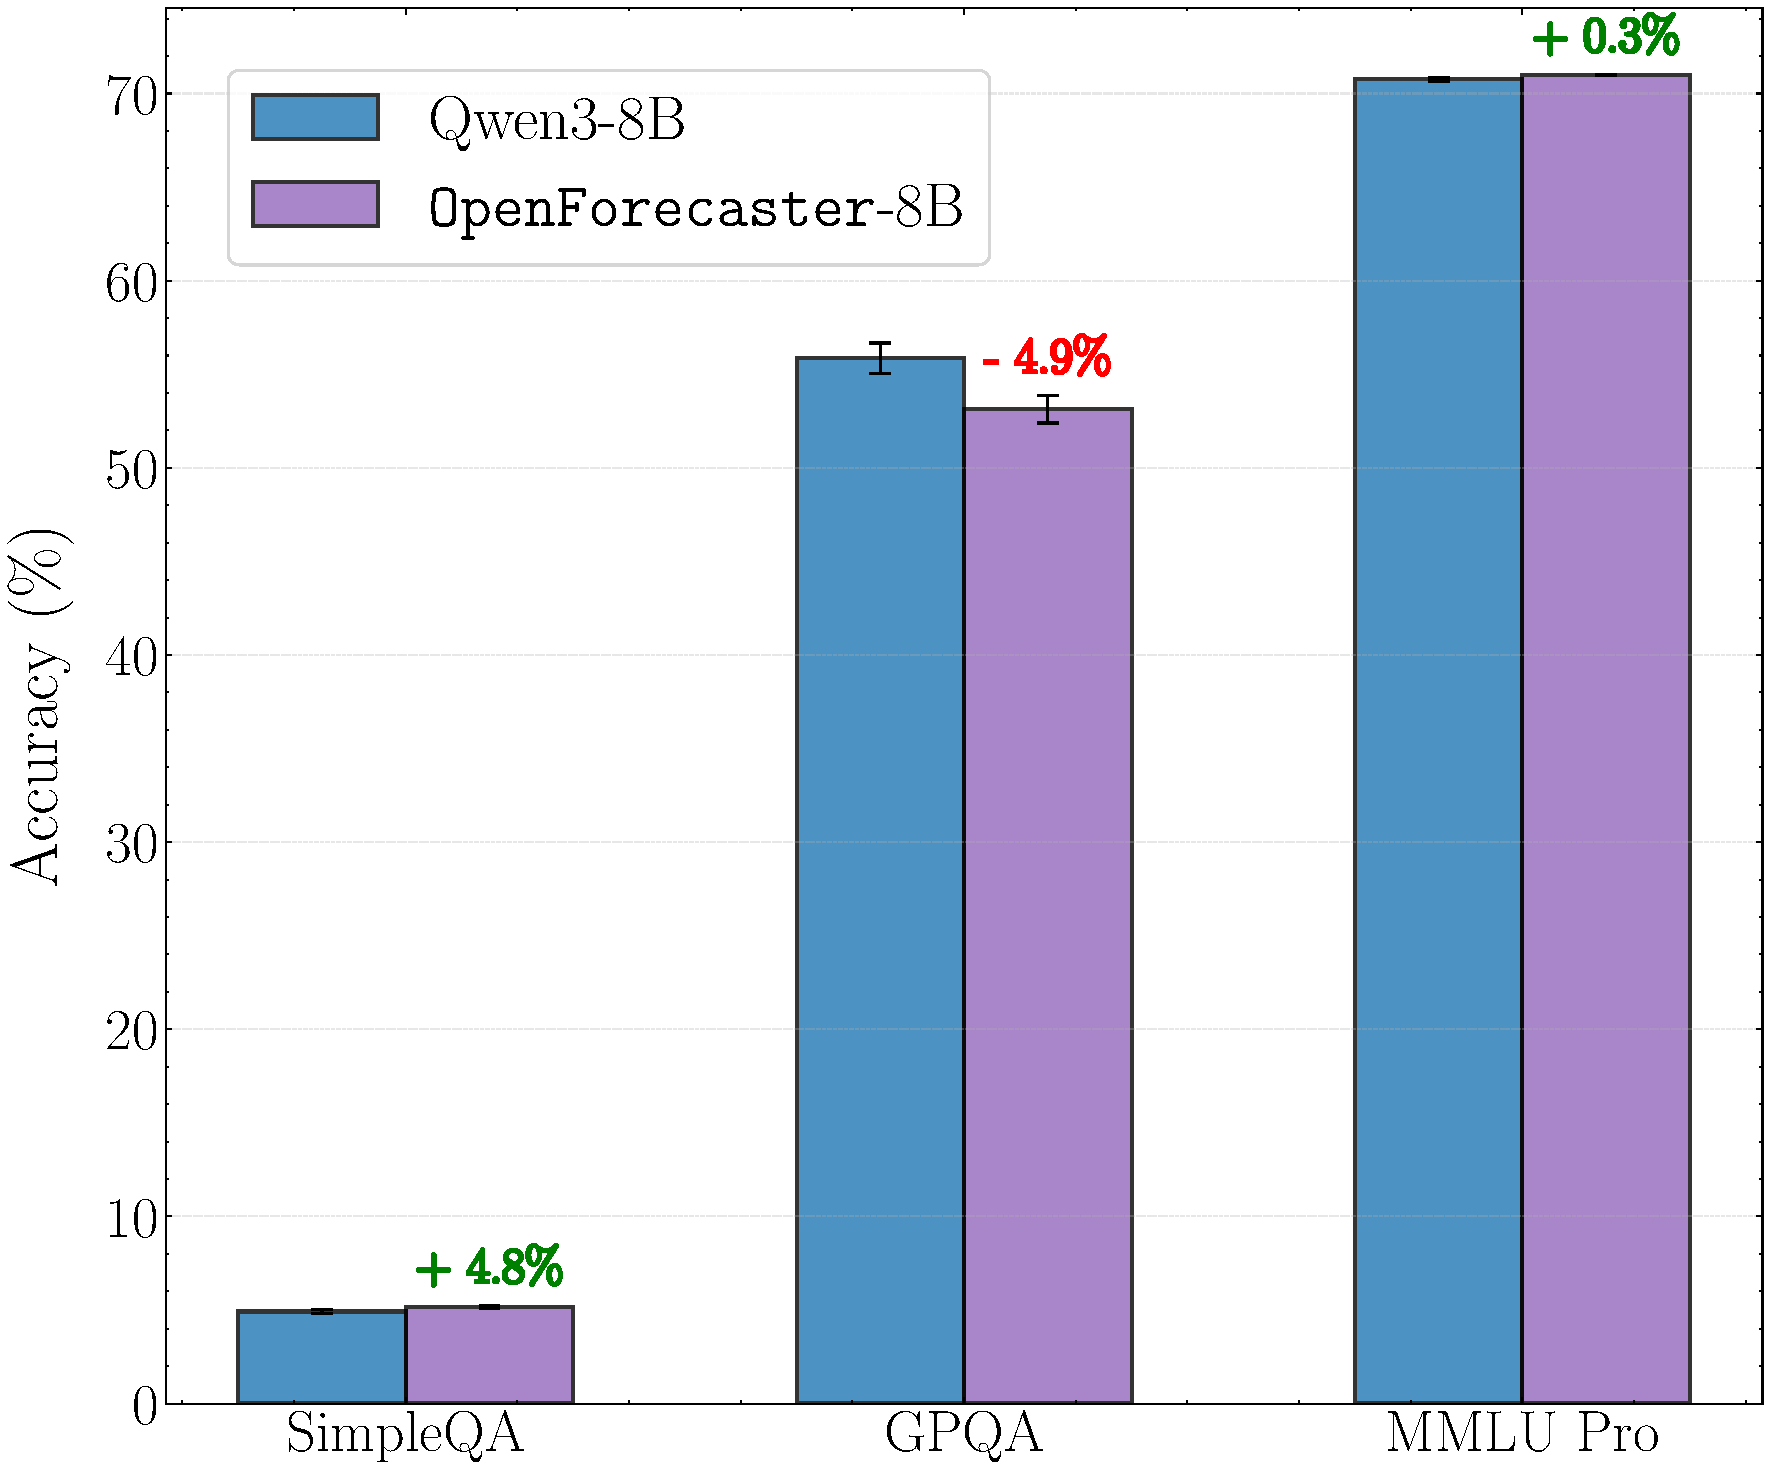
\includegraphics[width=0.95\linewidth]{figures/otherbenchmarks/accuracy_comparison.pdf}
        \caption{Accuracy comparison on general benchmarks. The number highlighted in green (red) shows \emph{relative} improvement (degradation) over the pre-RL model.}
        
        % \caption{{Accuracy of the models on FutureX Past.} }
        % \label{fig:futurex_acc}
         % latex is overrating the gap
    \end{minipage}
    % \caption{Performance of models from Llama and Gemma family our test set.} 
    \label{fig:accuracy_otherbenchmarks}
\end{figure}

% \vspace{-.2cm}
% \paragraph{Result 3: SFT improves pass@k performance of the model.} \Cref{fig:sft_passk} shows pre and post-SFT pass@k results. We observe SFT consistently improves both pass@1 and pass@k accuracy, ensuring little diversity collapse. We thus decide to use SFT to distill Grok-3-mini reasoning traces into our Qwen3-8B  model before further RL training.

\subsection{Evaluation on Metaculus Questions}
\label{sec:metaculus_results}


\begin{wrapfigure}[21]{r}{0.5\textwidth} % 'r' for right, 0.4\textwidth for width of figure area
    % \vspace{-0.4cm}
    \centering
    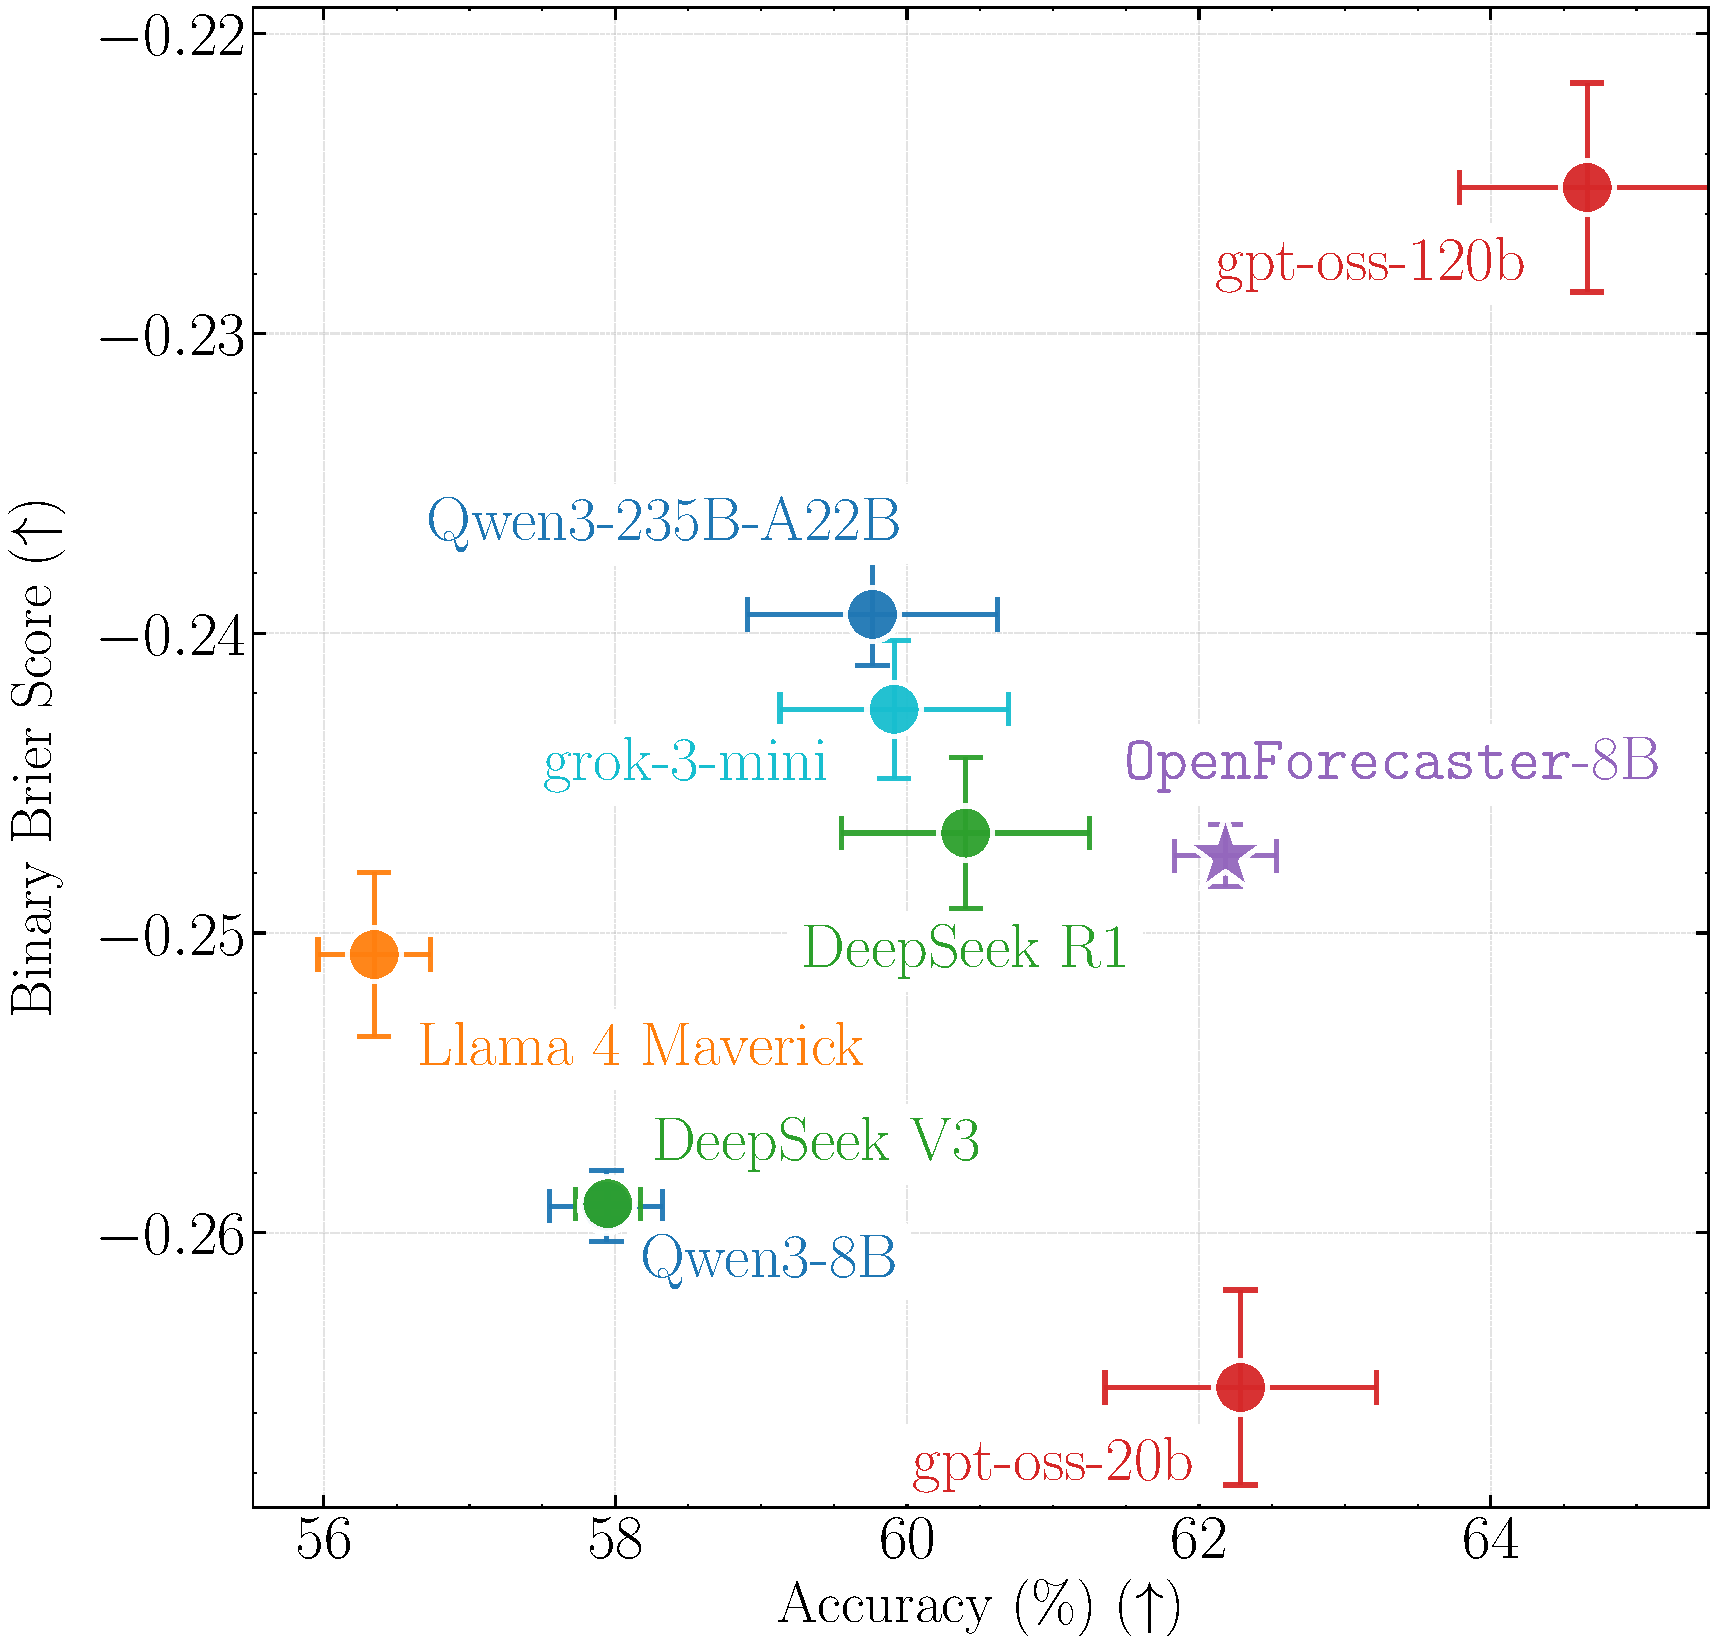
\includegraphics[width=\linewidth]{figures/metaculus/scatter_binary_brier_accuracy_metaculus_metaculusFromMayTillNov_30pdf.pdf}
    \caption{Performance of models on Metaculus questions from May 01 to Nov. 18 2025. 
    % \textbf{Improvement on brier score across OOD-benchmarks.} Our models significantly improve brier score (which jointly measures both accuracy and calibration) across diverse benchmarks.
    }
    \label{fig:metaculus_performance}
    \vspace{-.2cm} % latex is overrating the gap
    % \vspace{-.2cm} % latex is overrating the gap
\end{wrapfigure} 


\paragraph{Prediction Market Dataset.} We also source questions from the Metaculus prediction market from May - Nov. 2025. We filter questions which are either meta-prediction questions (prediction about some other prediction question on Metaculus), stock price prediction or below a certain trading volume leaving 449 high-interest questions. Each question is binary so a naive baseline gets 50\% accuracy. We evaluate models on this benchmark by computing both accuracy and brier score.


% \paragraph{Results of live evaluation on Metaculus.} 
% Finally, we also simulate live-testing of our frozen checkpoints from September on Metaculus from October 01 to November 18 2025. In this time window, we obtain 160 questions in from the Metaculus API. We filter questions which were related to stock price prediction, or meta-prediction about how Metaculus questions would resolve, as this requires access to very recent information not supported by our local offline news retrieval which is updated on a monthly cadence. This left us with $69$ samples. 
\paragraph{Results on Real Market Questions.} As shown in \Cref{fig:metaculus_performance}, \ourmodel \ 8B performs better than many larger models like DeepSeek-R1 and Llama-4-Maverick while GPT-OSS-120B is significantly better than rest of the models. \textbf{Note:} The brier score reported here is the \emph{standard brier score} used in prediction markets ranging from $-1$ to $0$ (with -0.25 being the baseline for a constant prediction of $50\%$) and this is different from the brier score we have reported earlier for freeform questions. 
